We had two possible implementations for the application layer. Had we chosen to do the processing in the cloud, the application layer would have just been a web interface for the user to interact with the system.

\subsection{Interface Subsystem}
The application layer handles communication with the rest of the system. More specifically, the Computer layer. Internally, it communicates with the data processing module and it receives information from the GUI as well.

\begin{figure}[h!]
	\centering
 	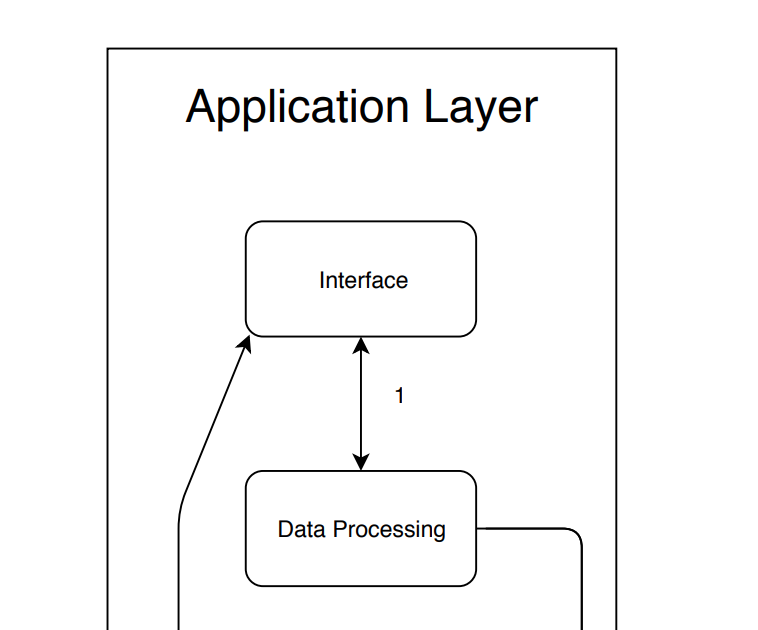
\includegraphics[width=0.60\textwidth]{images/app_sub_1}
 \caption{Interface Subsystem Diagram}
\end{figure}

\subsubsection{Assumptions}
It will receive data from the Computer layer.

\subsubsection{Responsibilities}
As previously stated, the application layer main interface handles communication from the Computer layer. It takes as input raw video from the computer layer and it passes it on to the data processing module. The main interface is synonymous with the graphical user interface which is just the visual representation of data for our system with an added layer of abstraction.

\subsubsection{Subsystem Interfaces}

\begin {table}[H]
\caption {App interface subsystem interfaces} 
\begin{center}
    \begin{tabular}{ | p{1cm} | p{6cm} | p{3cm} | p{3cm} |}
    \hline
    ID & Description & Inputs & Outputs \\ \hline
    \#0 & Handles communication between the application layer and the rest of the system & \pbox{3cm}{warning messages \\ Data} & \pbox{3cm}{Pre-processed video}  \\ \hline
    \end{tabular}
\end{center}
\end{table}


\subsection{Data Processing Subsystem}
This modules simply takes video as input and outputs an analyzed/condensed version of the input.

\begin{figure}[h!]
	\centering
 	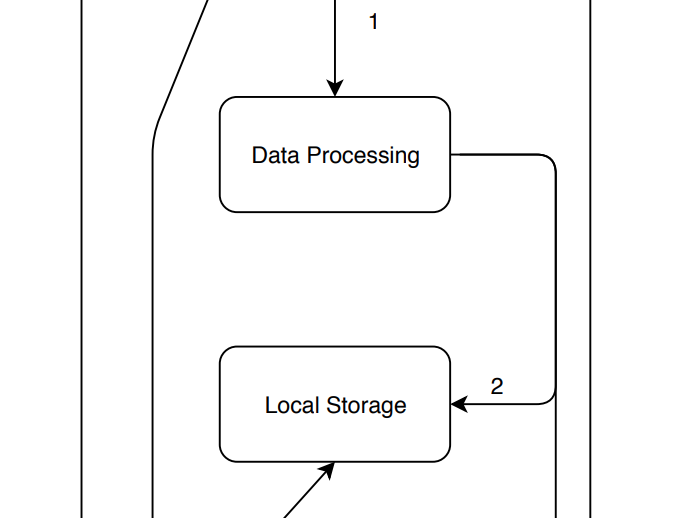
\includegraphics[width=0.60\textwidth]{images/app_sub_2_1}
 \caption{Data processing subsystem Diagram}
\end{figure}

\subsubsection{Assumptions}
The Computer layer completed the pre-processing successfully.

\subsubsection{Responsibilities}
This subsystem handle putting the bounding boxes around every vehicle along with measuring and recording the speed of every vehicle that the system deems to be appropriate. The data processing module also filters out anything that is not a vehicle.

\subsubsection{Subsystem Interfaces}

\begin {table}[H]
\caption {Data processing subsystem interfaces} 
\begin{center}
    \begin{tabular}{ | p{1cm} | p{6cm} | p{3cm} | p{3cm} |}
    \hline
    ID & Description & Inputs & Outputs \\ \hline
    \#1 & Handles the video processing & \pbox{3cm}{pre-processed video} & \pbox{3cm}{processed video \\ Analytics}  \\ \hline
    \end{tabular}
\end{center}
\end{table}

\subsection{Local Storage Subsystem}
Archives the analyzed video from the data processing module.

\begin{figure}[h!]
	\centering
 	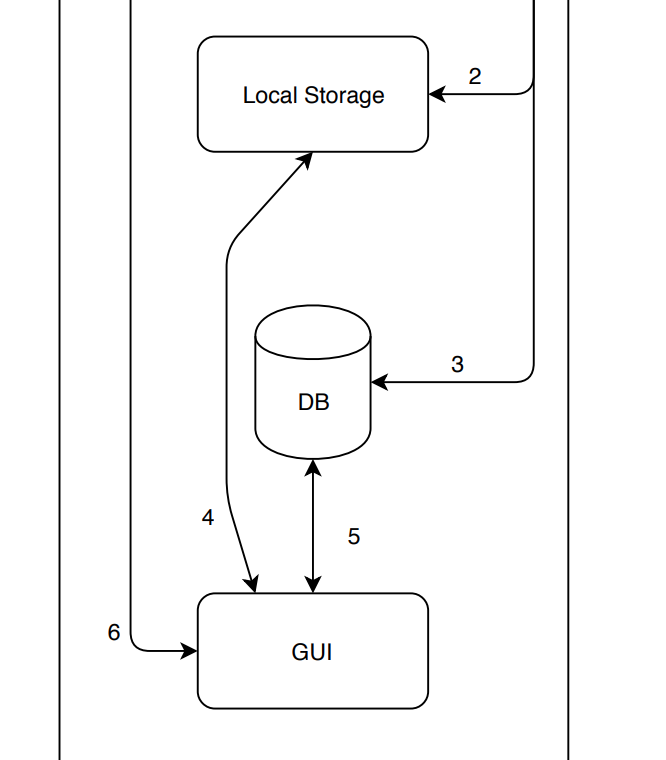
\includegraphics[width=0.60\textwidth]{images/app_sub_3}
 \caption{Local Storage subsystem Diagram}
\end{figure}

\subsubsection{Assumptions}
There will be sufficient local storage available.

\subsubsection{Responsibilities}
Simply archives the analyzed video from the data processing module so that the user has access to it from the GUI.

\subsubsection{Subsystem Interfaces}

\begin {table}[H]
\caption {Local Storage subsystem interfaces} 
\begin{center}
    \begin{tabular}{ | p{1cm} | p{6cm} | p{3cm} | p{3cm} |}
    \hline
    ID & Description & Inputs & Outputs \\ \hline
    \#2 & Archives analyzed video & \pbox{3cm}{Processed video \\ error messages} & \pbox{3cm}{processed videos}  \\ \hline
    \end{tabular}
\end{center}
\end{table}

\subsection{Database Subsystem}
A local database that archives analytics from the traffic study that is being conducted.

\begin{figure}[h!]
	\centering
 	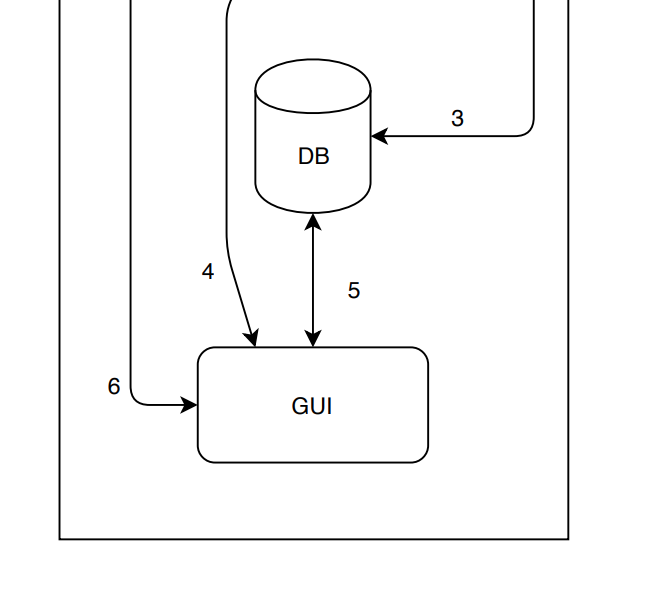
\includegraphics[width=0.60\textwidth]{images/app_sub_4}
 \caption{Database subsystem Diagram}
\end{figure}

\subsubsection{Assumptions}
It can be hosted on the local machine.

\subsubsection{Responsibilities}
The database takes data in from the data processing module. The GUI will be able to pull information from the database.

\subsubsection{Subsystem Interfaces}

\begin {table}[H]
\caption {Database subsystem interfaces} 
\begin{center}
    \begin{tabular}{ | p{1cm} | p{6cm} | p{3cm} | p{3cm} |}
    \hline
    ID & Description & Inputs & Outputs \\ \hline
    \#3 & Archives data from the traffic study & \pbox{3cm}{Processed data \\ Action from GUI} & \pbox{3cm}{Data for GUI}  \\ \hline
    \end{tabular}
\end{center}
\end{table}

\subsection{Graphical User Interface Subsystem}
The graphical user interface will allow the user to interact with the system. 

\begin{figure}[h!]
	\centering
 	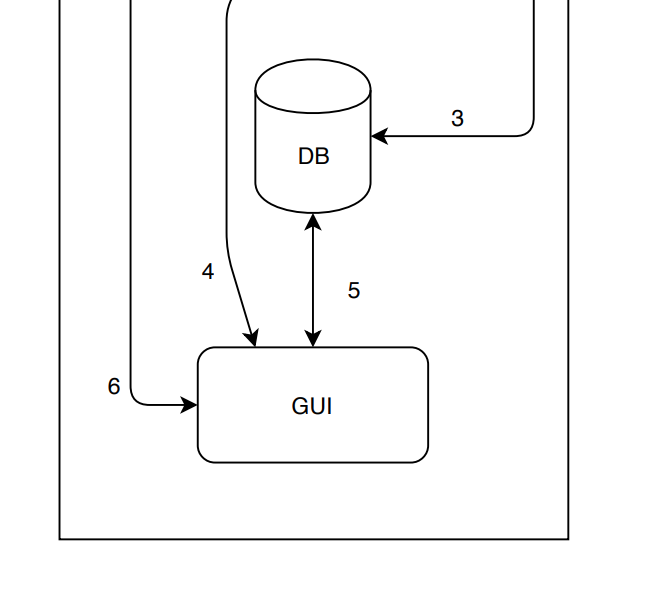
\includegraphics[width=0.60\textwidth]{images/app_sub_4}
 \caption{GUI Subsystem Diagram}
\end{figure}

\subsubsection{Assumptions}
The rest of the application layer functions properly.

\subsubsection{Responsibilities}
The user will be presented with a few options. They will be able to configure a few system options like setting the recording time intervals. They will have the option to be presented with a dashboard that has the visual representations of all the data in the form of graphs and tables. The user will also be able to see the recorded video and to start a new traffic study which deletes old data/video.

\subsubsection{Subsystem Interfaces}

\begin {table}[H]
\caption {Graphical User Interface Subsystem interfaces} 
\begin{center}
    \begin{tabular}{ | p{1cm} | p{6cm} | p{3cm} | p{3cm} |}
    \hline
    ID & Description & Inputs & Outputs \\ \hline
    \#4,5,6 & Allows the user to interact with the system & \pbox{3cm}{Data about system status \\ Current local storage space, videos \\ Data from DB} & \pbox{3cm}{Error messages \\ Data deletion option for both LS and DB}  \\ \hline
    \end{tabular}
\end{center}
\end{table}



